\newcommand{\problembox}[3]{
    \begin{table}[H]
        \centering
        \begin{tabularx}{\textwidth}{|Xr|}
            \hline
            #1 & #2 \\ \hline
            \multicolumn{2}{|>{\hsize=\dimexpr2\hsize+2\tabcolsep+\arrayrulewidth\relax}X|}{#3} \\ \hline
        \end{tabularx}
    \end{table}
}

\lstset{
    language=C++, % choose the language of the code
    basicstyle=\footnotesize\ttfamily, %\color{red},
	keywordstyle=\color{blue}\ttfamily,
    stringstyle=\color{red}\ttfamily,
    commentstyle=\color{gray}\ttfamily,
    extendedchars=false,
    numbers=left, % where to put the line-numbers
    numberstyle=\tiny, % the size of the fonts that are used for the line-numbers     
    showspaces=false, % show spaces adding particular underscores
    showstringspaces=false, % underline spaces within strings
    showtabs=false, % show tabs within strings adding particular underscores
    frame=single, % adds a frame around the code
    tabsize=2, % sets default tabsize to 2 spaces
    captionpos=b, % sets the caption-position to bottom
    breaklines=true, % sets automatic line breaking
    breakatwhitespace=false, 
}


\title{圖論}

\author{李昕威} %作者
\date{8th, February 2021}
\lfoot{Author:~\theauthor}
\maketitle
\thispagestyle{fancy}

\section{摘要}

  圖論中的圖並非指照片或圖片,而是由一些點和邊所組成。藉由這些點和邊,我們可以用其來研究物體之間的關係。舉例來說,可以將人視為點,如果兩個人互為朋友的話則將兩個點連上一條邊,這樣就構成了一張交友關係的圖。

在本章節中,我們會介紹圖論的基本名詞、圖的表示法、圖的遍歷、最短路徑、樹與其前中後序、最小生成樹。如果時間允許的話,我們會也會介紹有向無環圖、二分圖。最後一章的佛洛伊德演算法為科展性質的主題,有興趣鑽研的人再看即可。

\section{名詞介紹}
圖$G$是由節點$V$與邊$E$所組成,記做$G=(V, E)$。

\hspace*{\fill}

*和圖相關的名詞:
\begin{enumerate}
\item 有向圖:圖中的邊皆為有向邊。
\item 無向圖:圖中的邊皆為無向邊。
\item 簡單圖:一個不含重邊和自環的無向圖。
\end{enumerate}

\hspace*{\fill}

*和節點相關的名詞:
\begin{enumerate}
    \item 相鄰:若兩個點$u$、$v$之間有邊相連,則稱$u$、$v$相鄰。
    \item 度數:無向圖中,一個點所連的邊的數量,記做$deg(u)$。
    \begin{enumerate}
        \item 入度:有向圖中,一個點連「入」的邊的數量,記做$deg^+(u)$。
        \item 出度:有向圖中,一個點連「出」的邊的數量,記做$deg^-(u)$。
    \end{enumerate}
\end{enumerate}

\hspace*{\fill}

*和邊相關的名詞:
\begin{enumerate}
\item 權重:邊上的數值,可以用來代表長度、費用...等等。
\item 重邊:起點與終點相同的兩條邊。
\item 路徑:給定起點$x$和終點$y$,由$x$出發,沿著邊走到$y$,途中經過的邊構成的序列稱為路徑。
\item 環:一條路徑的起點與終點若為相同的點,則稱為環。由一條邊組成的環稱為自環。
\item 連通:點$A$與點$B$是連通,表示存在一條路徑由$A$走到$B$。
\end{enumerate}

\section{圖的表示法}

  在資訊的領域中,儲存資料的方法非常重要,甚至會影響到演算法的執行時間。
\hspace*{\fill}

以下將會介紹兩種存圖的方法:相鄰矩陣、鄰接串列。

\subsection{相鄰矩陣}

  開一個二維陣列存邊,兩個維度分別為起點和終點的節點編號。如果圖上的邊沒有權重,通常使用bool陣列存節點$i,j$之間有沒有邊。如果圖上的邊有權重,通常使用int陣列存節點$i,j$之間的權重,如果$i,j$間不存在邊,通常以INF表示。

\hspace*{\fill}

\begin{lstlisting}[caption=相鄰矩陣]
#include <bits/stdc++.h>
using namespace std;
int n, m;
int G[2009][2009];
int main() {
	cin >> n >> m;
	for (int i = 0; i < m; ++i) {
		int a, b, c;
		cin >> a >> b >> c;
		G[a][b] = c;
		//G[b][a] = c; 無向圖的話要加上這一行
		//可以想想看沒有邊權的情況是如何?
	}
}
\end{lstlisting}

\begin{table}[ht]
\centering
    \begin{tabular}{c|cccccc}
           & A & B & C & D & E & F \\ \hline
         A & INF & 4 & 2 & INF & INF & INF \\ 
         B & INF & INF & 5 & 10 & INF & INF \\
         C & INF & INF & INF & INF & 3 & INF \\
         D & INF & INF & INF & INF & INF & 11 \\
         E & INF & INF & INF & 4 & INF & INF \\
         F & INF & INF & INF & INF & INF & INF \\
    \end{tabular}
\caption{以相鄰矩陣表示圖}
\end{table}

這個方法的空間複雜度為$O(V^2)$,因此當點數大於$5000$之後,通常不會以這種方法存圖。另外,使用這個方法時,也必須小心處理重邊、初始化的問題。

綜上所述,實際上使用這種方法來存圖的情況較少。

\subsection{相鄰串列}

  對於每一個點,儲存以此點為起點的邊。通常對每個點,使用一維vector陣列儲存 。
\clearpage

\begin{table}[ht]
\centering
    \begin{tabular}{| m{1cm} | m{1cm} m{1cm} m{1cm} m{1cm} m{1cm}|} \hline
         1 & 2 & 3 & 4 & 5 & 6\\ \hline
         2 & 1 & 3 &  & &\\ \hline
         3 & 1 & 2 & 5 &  &  \\ \hline
         4 & 1 & 5 &  &  &  \\ \hline
         5 & 1 & 3 & 4 &  &  \\ \hline
         6 & 1 &  &  &  &  \\ \hline
    \end{tabular}
\caption{以相鄰矩陣表示圖}
\end{table}

\begin{lstlisting}
#include <bits/stdc++.h>
using namespace std;

int n, m;
vector<int> v[1000009];

int main() {
	cin >> n >> m;
	for (int i = 0; i < m; ++i) {
		int a, b;
		cin >> a >> b;
		v[a].push_back(b);
		//v[b].push_back(a); 無向圖的時候要加上這一行
	}
}
\end{lstlisting}

\hspace*{\fill}

若要儲存帶邊權的圖的話,則可以藉由\verb|vector<pair<int,int>>|來完成。

\hspace*{\fill}

\begin{lstlisting}
#include <bits/stdc++.h>
using namespace std;

int n, m;
vector<pair<int,int> > v[1000009];

int main() {
	cin >> n >> m;
	for (int i = 0; i < m; ++i) {
		int a, b, w;
		cin >> a >> b >> w;
		v[a].push_back(make_pair(b, w));
		//v[b].push_back(make_pair(a, w)); 無向圖的時候要加上這一行
	}
}
\end{lstlisting}

鄰接串列的空間複雜度為$O(V+E)$。

使用相鄰矩陣的優點是可以$O(1)$判斷兩點是否相鄰,而相鄰串列的話則必須要對每個vector進行sort後二分搜,因此時間複雜度為$O(VlogV)$預處理、$O(logV)$查詢。但相鄰矩陣的空間複雜度實在過大,因此大多數情況下還是使用相鄰串列。

\section{圖的遍歷}

  圖的遍歷基本上有兩種方法,深度優先搜尋DFS、廣度優先搜尋BFS。

在遍歷圖的過程中,我們會從一個節點轉移到另一個節點。很多人會卡住的原因是:不知道程式碼要填什麼。在此建議從搜尋到一半的狀態開始想像:

\begin{enumerate}
\item 目前狀態:到了一個節點後,這個點的狀態要從「未處理」標記成「處理中」。
\item 轉移:可以轉移到哪些狀態?
\item 結束:點的狀態由「處理中」改為「完成」。
\end{enumerate}

\subsection{深度優先搜尋 DFS}

  DFS顧名思義,是有路的話就一直往下走,一直走到死路後再回頭,並選擇其它可以走的路,繼續試著往下走。

\begin{lstlisting}[caption=DFS範例]
#include <bits/stdc++.h>
using namespace std;

bool[1000009] visited;
vector<int> v[1000009];

void dfs(int u) {
	visit[u] = 1;
	for (auto i:v[u]) if (!visited[i]) {
		dfs(i);
	}
}
\end{lstlisting}

要記得將走過的地方標記起來,以免下次再走。

DFS 較常用來枚舉與順序性有關的題目,如:排列組合(誰坐誰不坐)、一筆劃問題。

\subsubsection{例題演練}

\problembox{一筆劃問題}{UVA 291}{
\begin{minipage}{0.6\textwidth}
由小到大輸出右圖所有由$1$開始經過所有邊的走法,第一組是$123153452$,最後一組是$154352312$。(註:uva上範例輸出有誤)
\end{minipage}
}

  解題的第一步是將圖建出來,題目要求要依照大小輸出,如果使用相鄰串列可事先將邊依照節點的編號由小到大排序。接著用dfs的方式枚舉不重複邊的走法,並且紀錄當前走法依序經過哪些節點。當遞迴到底時表示這個走法已經經過所有邊,因此輸出這組走法。

\subsubsection{練習題}

\problembox{1.銀河帝國旅行社}{TIOJ 1152}{
    給你一顆至多有$10^4$個點的樹,請問樹上最遠的兩個點間的距離是多少。
}

\problembox{Destruction of a Tree}{CF 963B}{
    給你一顆至多$2\times 10^5$個節點的樹,一個點可以被摧毀若且唯若它的度數為偶樹,且一個點被摧毀後,它所連接出去的邊也會跟著被摧毀,請問能不能摧毀掉整顆樹,如果可以,請輸出摧毀的順序。
    
    (hint:可以將節點數為偶數和奇數的情況分開考慮)
}

\problembox{數獨問題}{TIOJ 1025}{
    給你一個未完成的數獨,請輸出所有可能的答案。
    
    (hint:雖然乍看之下會TLE,但其實只要好好檢查發生矛盾的情況就可以很快跑出結果來的)
}

\subsection{廣度優先搜尋 BFS}

  BFS的搜索過程可以想像成是將水倒在起點,這時水會以等速率向四周擴散。BFS也是同個道理,BFS先搜尋$n$步可以走到的點後,再搜尋$n+1$步可以走到的點,以此類推。

\begin{lstlisting}[caption=BFS範例]
#include <bits/stdc++.h>
using namespace std;

bool visited[1000009];
vector<int> v[1000009];
queue<int> q;

int main() {
	q.push(1); //假設1為起點
	while (q.size()) {
		int u = q.front();
		q.pop();
		for (auto i:v[u]) if (!visited[i]) {
			visited[i] = 1;
			q.push(i);
		}
	}
}
\end{lstlisting}

每走到一個點後,就將其周圍還沒走到的點都放去queue的最後面,這樣就能保證離原點較近的點會先被走到。此外,已經放進queue裡的點要標記起來,以免重複放進queue裡。

\subsubsection{例題演練}

\problembox{水桶問題}{UVA 571}{
有兩個水桶A,B,容量分別為$C_a, C_b$,求如何操作可以得到N公升的水(位於A或B水桶皆可)。
一開始兩個水桶都是空的。
以下幾種操作:
\begin{enumerate}
\item 裝滿A
\item 裝滿B
\item 清空A
\item 清空B
\item A倒滿B(不溢出)
\item B倒滿A(不溢出)
\end{enumerate}
}

  以兩水桶水量當作狀態,每個狀態最多可以再延伸出6個狀態,可以建出一張狀態圖。不難發現這題要找的是此狀態圖中,從「A,B都是0」這個節點到「A,B其中一個是N」這個節點的路徑。我們可以用BFS的方式找出這條路徑。

\subsection{練習題}

\problembox{Fire in the forest}{TIOJ 1013}{
    給你一張$17\times 10$的棋盤圖,有些格子上著火了,若一個格子的上下左右有任何一個格子著火,那麼下一秒它也會跟著著火。你走路的速度為一秒一格,現在給你你的起點位置和目的地,還有目前棋盤的著火情況,請問你能夠成功到達目的地嗎?
}

\problembox{量杯問題}{TIOJ 1008}{
    你有最多五個有著整數容量的量杯,請問是否能用這些量杯量出$L$公升的水。
    
    (hint:這題是經典的將狀態當作圖的節點的例子,但這題的狀態頗多,需要壓縮狀態的技巧)
}

\section{最短路徑 Shortest Path}

  在一張圖上若兩點之間互不連通,則定義其距離為無限大;反之則定義為所有路徑之中,邊權和最小的那一個,也就是所謂的最短路徑。

\subsection{BFS}
  首先考慮所有邊的邊權都一樣的情況,這樣一來很自然地就會想到使用BFS,由於在queue中的節點都保證了先被放進去的肯定比後放進去的,離起點的距離更近,因此BFS就可以解決了。

\subsubsection{練習題}

\problembox{三維迷宮問題}{TIOJ 1085}{
    給你一個三維棋盤狀的迷宮,長寬高皆小於50,0代表可以走、1代表不能走的地方,請問從$(0, 0, 0)$走到對角線的那個最遠點的最短距離是多少。
}

\problembox{H.跑跑卡恩車}{TIOJ 1022}{
    在一張長寬皆小於100的棋盤上,相鄰兩格間能相通若且唯若兩格的數字差$\leq$5,請問從左上角走到右下角的最短距離為何。
}

\subsection{鬆弛}
  求最短路徑問題有個非常重要的核心概念,稱之為鬆弛:若目前$a$到$b$的距離大於$a$到$c$再從$c$到$b$的距離的話,則將其更新為較小值,即:

\begin{center}
    \lstinline{d[a][b] = min(d[a][b], d[a][c]+d[c][b])}。
\end{center}

\subsection{Dijkstra}

  Dijkstra是單點源最短路徑演算法,其核心概念為貪心法:每次挑選一個離起點最近的點,將其標記為「確認了最短路徑的點」後,利用這個點去鬆弛起點與其他「還沒確認最短路徑的點」的距離,再從「還沒確認最短路徑的點」中挑出一個離起點最近的點,重複這樣的動作。

特別注意:上述性質成立的條件是圖上\textbf{不存在邊權為負的邊},因此Dijkstra\textbf{不適用於有負邊的圖}。

\begin{lstlisting}[caption=Dijkstra演算法]
using pii = pair<int, int>;
int n, m;
vector<pii> v[1000009];
priority_queue<pii, vector<pii>, greater<pii> > pq;
int d[1000009];

void dijkstra() { // 假設起點為1
	for (int i = 2; i <= n; ++i) d[i] = 1e9;
	pq.push(mk(d[1], 1)); // (距離, 點)
	
	while (pq.size()) {
		auto u = pq.top();
		pq.pop();
		if (d[u.second] != u.first) continue;
		
		for (auto i : v[u.second]) {
			if (d[i.first] > u.first + i.second) {
				d[i.first] = u.first + i.second;
				pq.push(make_pair(d[i.first], i.first));
			}
		}
	}
}
\end{lstlisting}

首先要記得將除了起點以外的點和起點的距離設定為無限大,pq裡存的為每次選到的距離最近的點。但因為同個點可能會被鬆弛很多次,所以若是選到了一個「距離比『真正的距離』大」的點的時候,代表那個點已經被其他點鬆弛過了,因此就必須忽略這次。

這個演算法的複雜度為$O(E\log E)$。

\subsubsection{練習題}

\problembox{F.不定向邊}{TIOJ 1209}{
    給你一張點數少於$10^3$、邊數少於$10^6$的帶權(非負整數)圖,在可以自由指定每條路的方向下,請問從起點到終點的最短路徑為多少。
}

\problembox{地道問題}{TIOJ 1509}{
    給你一張有向帶權圖,點數邊數$\leq 10^6$,對於每個點求從起點走到它再走回起點的最小距離,再把所有點的答案加總。
    
    (hint:可不是直接從起點做$dijkstra$加總後乘兩倍,因為回來的時候能走的路和去的時候不一樣)
}

\problembox{貨物運送計劃}{TIOJ 1641}{
    給定一張點數少於$10^4$、邊數少於$2\times 10^5$的無向帶權(正整數)圖,並給定起點與終點,一開始在起點時你有$1$個東西,每經過一條邊權為$P_i$的點,你身上的東西就會變成(你現在有的東西數量)$\times P_i$,請問到達終點時你身上最少有多少東西。
}

\subsection{Bellman-Ford}

  Bellman-Ford是另一種單點源最短路徑演算法,相對於Dijkstra,Bellman-Ford藉由每次檢查每條邊是否能夠鬆弛其端點,若沒有則代表找到了所有點的最短路;若是一個點被鬆弛了超過$V$次,就代表此圖存在負環。

\begin{lstlisting}[caption=SPFA演算法]
using pii = pair<int, int>;
int n, m;
bool inque[1000009];
vector<pii> v[1000009]; 
queue<int> q;
int d[1000009], cnt[1000009];

bool SPFA() {
	for (int i = 2; i <= n; ++i) d[i] = INF;//初始化距離
	q.push(1); //假設起點為 1
	inque[1] = 1;
	d[1] = 0;
	while (q.size()) {
		int u = q.front();
		q.pop();
		inque[u] = 0;
		for (auto i : v[u]) {
    		if (d[i.first] > d[u] + i.second) { //只需要處理將會被更新的點
    		    cnt[i.first] += 1;
    			if (cnt[i.first] >= n) return false; //發現負環
    			d[i.first] = d[u] + i.second;
    			if (!inque[i.first]) {
    				inque[i.first] = 1;
    				q.push(i.first);
    			}
    		}
		}
	}
	return true; //沒有負環
}
\end{lstlisting}


SPFA演算法全名Shortest Path Faster Algorithm,是Bellman-Ford的優化。SPFA把更新過的節點放入一個Queue,並且只檢查Queue中的邊。在隨機生成的圖上,平均每個節點被更新兩次,期望複雜度為$O(2E)$。

但最差的時間複雜度為$O(VE)$,而且很容易可以構造出會跑到$O(VE)$的測資。

\subsection{Floyd-Warshall}

  重新看看鬆弛的算式:\lstinline{d[a][b] = min(d[a][b], d[a][k]+d[k][b];},是不是很像DP呢?

\hspace*{\fill}

若將DP的狀態設為:

\begin{center}
    \lstinline{dp[k][i][j]}
\end{center}

代表從$i$走到$j$並且經由前$k$個節點鬆弛過後的結果,那麼轉移式就是:


\begin{center}
    \lstinline{dp[k+1][i][j] = min(dp[k][i][j], dp[k][i][k+1] + dp[k][k+1][j])}
\end{center}

\hspace*{\fill}

觀察一下發現討論$k+1$時只會用到$k$的部份,因此我們可以滾動dp陣列。


\clearpage

\begin{lstlisting}[caption=floyd warshall]
int dp[N][N];
for (int k = 0; k < N; ++k)
  for (int i = 0; i < N; ++i)
    for (int j = 0; j < N; ++j)
      dp[i][j] = min(dp[i][j], dp[i][k] + dp[k][j]);
\end{lstlisting}

Floyd-Warshall的時間複雜度為$O(V^3)$,然後可以$O(1)$查詢任一點對的最短距離。

另外,這是一個需要用到鄰接矩陣的例子。

\subsubsection{練習題}

\problembox{搶救雷恩大兵}{TIOIJ 1034}{
    給 $N \times N (\leq 20)$ 的棋盤圖,每個棋盤上的點都有權值。$Q(\leq N^4)$筆詢問兩個點的路徑中,可以把一個點的值改成 0 的狀況下,最小的總和是多少。
}

\problembox{圖論 之 最小圈測試}{TIOJ 1212}{
    給一張點數少於$5\times 10^2$的無向圖,邊權皆為一,請問長度最小的環的長度為多少?
}

\problembox{E.漢米頓的麻煩}{TIOJ 1096}{
    給一張點數至多為100的圖,一個點的花費為從自己經過一些不重複的路徑後回到自己的邊權和,請問所有點中最少的花費為何?
}

\section{樹}

樹的定義為一張沒有環的連通圖。

\begin{figure}[h!]
    \begin{minipage}{0.32\textwidth}
        \centering
        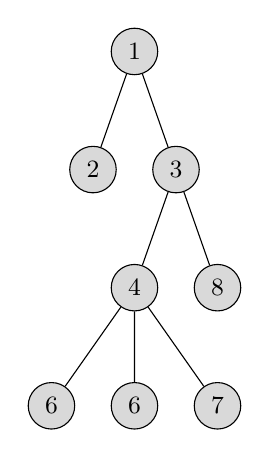
\begin{tikzpicture}[
            sibling distance=3em,
            every node/.style = {shape=circle, draw=black, fill=gray, fill opacity = 0.3, text opacity=1, align=center, font=\small}
          ]
          \node {1}
            child { node {2} }
            child { node {3}
                child { node {4}
                    child { node {6} }
                    child { node {6} }
                    child { node {7} } 
                }
                child { node {8} } 
            };
        \end{tikzpicture}
        \caption{樹}
    \end{minipage}
    \hfill
    \begin{minipage}{0.32\textwidth}
        \centering
        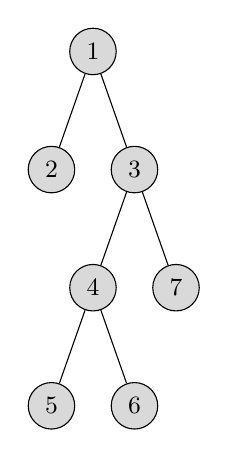
\begin{tikzpicture}[
            sibling distance=3em,
            every node/.style = {shape=circle, draw=black, fill=gray, fill opacity = 0.3, text opacity=1, align=center, font=\small}
          ]
          \node {1}
            child { node {2} }
            child { node {3}
                child { node {4}
                    child { node {5} }
                    child { node {6} }
                }
                child { node {7} } 
            };
        \end{tikzpicture}
        \caption{二元樹}
    \end{minipage}
    \hfill
    \begin{minipage}{0.32\textwidth}
        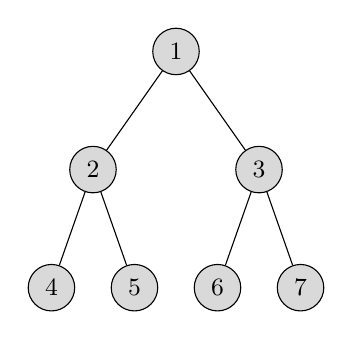
\begin{tikzpicture}[
            level 1/.style = {sibling distance=6em},
            level 2/.style = {sibling distance=3em},
            every node/.style = {shape=circle, draw=black, fill=gray, fill opacity = 0.3, text opacity=1, align=center, font=\small}
          ]
          \node {1}
            child { node {2}
                child { node {4} }
                child { node {5} } 
            }
            child { node {3}
                child { node {6} }
                child { node {7} }
            };
        \end{tikzpicture}
        \caption{完整二元樹}
    \end{minipage}
\end{figure}

\subsection{專有名詞與性質}

  以下為樹相關的名詞:

\begin{enumerate}
\item 根:樹的起點,根據是否有指定起點可分為有根樹和無根樹。
\item 父節點、子節點:遍歷樹的過程中,我們由父節點走向相鄰的子節點。
\item 葉節點:位於樹的盡頭,度數為1的點。
\item 祖先:由父節點到樹根路徑上的所有節點。
\item 子樹:分別以每個子節點為根的樹。
\item 層:一個節點與根的距離,根位在第0層。
\item 深度:整棵樹的層數,即從樹根到最遠的葉節點的路徑上經過的節點總數。
\end{enumerate}

\hspace*{\fill}

根據樹的定義,我們可以推導出一些樹的性質:

\begin{enumerate}
\item 一顆樹剛好$|V|-1$條邊。
\item 一顆樹沒有環,但加上任何一條邊都會出現環。
\item 一顆樹連通,且任何一條邊被拿掉都會導致圖不連通。
\item 一顆樹上任意兩點只存在一條簡單路徑。
\end{enumerate}

\subsubsection{二元樹的遍歷}

  二元樹的遍歷基本上分為以下四種。
\begin{enumerate}
    \item 前序:先走根,再走左子樹,最後走右子樹
    \item 中序:先走左子樹,再走根,最後走右子樹
    \item 後序:先走左子樹,再走右子樹,最後走根
    \item 層次:由上到下、由左到右遍歷
\end{enumerate}

如果你同時有著一棵二元樹的前序、中序,或者是中序、後序的話,那你就能夠確定這棵二元樹的結構。
若你只有一顆二元樹的前序、後序的話,就可能會分辨不出一個葉節點是左節點還是右節點。

\subsubsection{練習題}

\problembox{Problem C 二元搜尋樹 (TRVBST)}{TIOJ 1609}{
    現在有一顆空的二元搜尋樹,並按照順序插入一些數字,最後請輸出這棵樹的中序表示法。
}

\problembox{樹狀的堆積結構}{TIOJ 1204}{
    給你一顆點數至多為$10^3$的堆積(heap,實作priority\_queue的資料結構,也就是所有父節點都大於其子節點)的中序表示法,請輸出其前序表示。
}

\problembox{繁複的二元樹}{TIOJ 1107}{
    請問要將$N$個數字$1,2,...,N$表示成一棵二元搜尋樹,有多少種表示法?由於答案可能很大,因此輸出四捨五入後的科學記號即可。
}

\problembox{樹的三兄弟}{TIOJ 1108}{
    給定一棵樹的前序和中序表示法,請輸出後序表示法。
}

\problembox{樹論 之 好多星星 ver 1.3}{TIOJ 1215}{
    給你節點數$N$,請畫出節點數為$N$的二元樹,其中$N$小於64。
}

\problembox{APCS1050305 血緣關係}{zerojudge b967}{
    給你一顆樹,求直徑(最遠的兩個節點距離)。
}

\section{最小生成樹}

  生成樹為一棵包含圖上所有點的樹。一張圖上可能存在多種生成樹。最小生成樹為權重和最小的生成樹。

\begin{figure}[h!]
\centering
    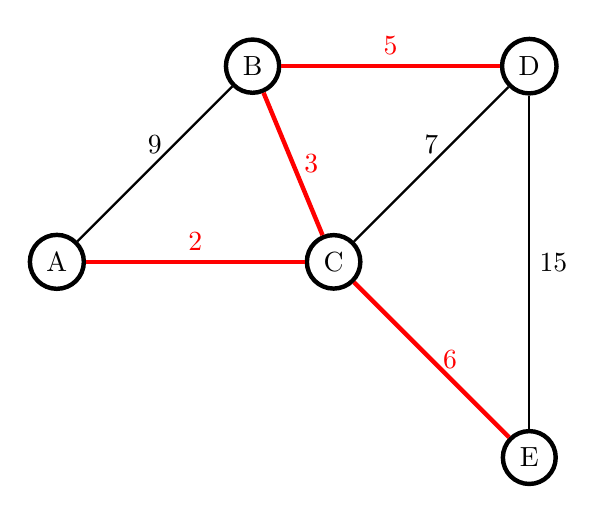
\begin{tikzpicture}[
        node distance = {10em}, 
        v/.style = {draw, ultra thick, circle},
        mst/.style = {color=red, ultra thick},
        e/.style = {thick}
    ]
    %--- Draw Vertices ---%
        \node (a) [v] {A};
        \node (b) [v, above right of = a] {B};
        \node (c) [v, right of = a] {C};
        \node (d) [v, above right of = c] {D};
        \node (e) [v, below right of = c] {E};
        %--- Draw MST ---%
        \draw[mst] (a) to node [above]{2} (c);
        \draw[mst] (b) to node [right]{3} (c);
        \draw[mst] (b) to node [above]{5} (d);
        \draw[mst] (c) to node [right]{6} (e);
        %--- Draw Edges ---%
        \draw[e] (a) to node [above]{9} (b);
        \draw[e] (c) to node [above]{7} (d);
        \draw[e] (d) to node [right]{15} (e);
    \end{tikzpicture}
\caption{圖上最小生成樹}
\end{figure}

舉例來說,電信公司佈線到每戶人家,但希望所用的電線越少越好,如果對每戶人家建圖,權重為兩戶間的距離,此時佈線的最佳辦法為圖上的最小生成樹。常見建構MST的演算法有兩種:以邊出發的Kruskal、以點出發的Prim。兩種都是以貪心的方式生成MST。

\subsection{Kruskal}

  由權重最小的邊開始加入生成樹,若目前選到的邊的兩端點都已經在生成森林中的同一棵樹時則略過。具體作法為將邊排序後,以disjoint set維護點是否在同一顆樹中,因此時間複雜度為$O(E\log E)$。

\clearpage

\begin{lstlisting}[caption=kruskal]
#include <bits/stdc++.h>
#define pii pair<int, int>
#define mk make_pair
#define F first
#define S second
using namespace std;

int n, m, ans;
vector<pair<int, pii> > G;

//省略Disjoint set

int main() { 
	cin >> n >> m;
	for (int i = 1; i <= m; ++i) {
		int a, b, w;
		cin >> a >> b >> w;
		G.pb(mk(w, mk(a, b)));
	}
	
	sort(G.begin(), G.end());
	for (auto i:G) if (!same(i.S.F, i.S.S)) {
		unite(i.S.F, i.S.S);
		ans += i.F;
	}
}
\end{lstlisting}

要注意的是,由於要對邊權排序,所以在這裡並不是使用鄰接串列來儲存圖,而是直接將每條邊存在vector裡面。

\subsection{Prim}

  回想Dijkstra是每次尋找離起點最近且還沒標記過的點,Prim其實就是每次尋找離目前的最小生成樹最近的點加進來。
  
\clearpage

\begin{lstlisting}[caption=prim]
#include <bits/stdc++.h>
#define pii pair<int, int>
#define mk make_pair
#define F first
#define S second
using namespace std;

int n, m;
bool visited[1000009];
vector<pi> v[1000009];
priority_queue<pii, greater<pii>, greater<pii> > pq;

int prim() {
	int ans = 0;
	visited[1] = 1;
	pq.push(make_pair(0, 1));
	while (pq.size()) {
		pi u = pq.top();
		pq.pop();
		if (visited[u.second]) continue;
		visited[u.second] = 1;
		ans += u.first;
		for (auto i:v[u.second]) {
			pq.push(i.second, i.first);// second代表邊權、first代表連到的點
		}
	}
	return ans;
}
\end{lstlisting}

在一般比賽裡,求生成樹的題目中點數和邊數基本上會是同個數量級,但kruskal的出場率遠遠比prim高,其原因就在於kruskal除了更容易理解外,實在是太好寫了。

\subsubsection{練習題}

\problembox{圖論 之 最小生成樹}{TIOJ 1211}{
    給一張點數至多$10^5$、邊數至多$10^6$的無向帶權圖,請求出最小生成樹的權重和。
}

\problembox{最小格子生成樹}{TIOJ 1326}{
    平面上給至多$10^3$個點,現在要用一些水平或垂直的線將所有點連在一起,請問這些線段的總長度最小為多少?
}

\problembox{黑色騎士團的番外野望 Dis-connect}{TIOJ 1596}{
    給你一棵點數至多為$10^5$的樹,拆掉一條邊的費用為其之上的邊權,其中有些點是軍事堡壘,請問至少要花多少錢才能使兩兩軍事堡壘不相通?
}

\problembox{咕嚕咕嚕呱啦呱啦}{TIOJ 1795}{
    給你一棵點數至多為$10^5$、邊數至多為$3\times 10^5$的圖,每條邊的邊權是一或者是零,沒有其他可能性,請問是否存在一棵生成樹的邊權恰好是$K$?
}

\section{二分圖}

二分圖顧名思義就是指,能夠將點分成$X$、$Y$兩類,使得同一類裡的點之間互相都沒有邊相連的圖。

\subsection{判斷一張圖是否為二分圖}

  二分圖有個等價定義為:不包含奇環的圖。若這一張圖中只包含了長度為偶數的環的話,那間隔的將點歸到X與Y內,自然就能滿足二分圖的定義;反之若有奇環的話,在那環上一定會有相鄰的兩點被放在同一類中。

所以判斷一張圖是否為二分圖的方法就不言自明了,利用DFS或BFS即可完成。

\begin{lstlisting}[caption=判斷是否為二分圖 範例]
#include<bits/stdc++.h>
using namespace std;

vector<int> v[1000009];
bool visited[1000009];
int col[1000009];

bool dfs(int x, int color) {
	bool isBip = 1;
	col[x] = color;
	visited[x] = 1;
	for (auto i:v[x]) {
		if (visited[i] && col[i] == col[x]) return false;
		if (!visited[i]) isBip &= dfs(i, color^1);
	}
	return isBip;
} 

int main() {
	int isBipartite = dfs(1, 1);
}
\end{lstlisting}

值得注意的是,上方的範例使用了color相關詞彙作為命名,這是因為在判斷二分圖的過程,有時候會習慣以將點染色來稱呼,相鄰兩點不能同色;另外,範例使用了XOR將要染的顏色在1與0間切換。

\subsection{練習題}

\problembox{圖論 之 二分圖測試}{TIOJ 1209}{
    給你一張點數最多為$4\times 10^4$、邊數最多為$5\times 10^5$的圖,請判斷這是不是一張二分圖。
}



\section{拓樸排序}

  給定一張有向無環圖(DAG),給每個點一個序號,總存在至少一個方式,使得所有序號大(小)的點不存在路徑到達序號小(大)的點,我們稱以這樣的序號排列出的點序列為拓撲排序。要構造的方法也很簡單,每次將出度為零的點push進一個stack(下方是以vector代替)中即可。

\clearpage

\begin{lstlisting}[caption=拓樸排序]
int n, m, deg[1000009];
vector<int> s, t, v[1000009];

vector<int> TopologicalSort() {
	for (int i = 1; i <= n; ++i) {
		if (deg[i] == 0) s.push_back(i);
		deg[i] = v[i].size();
	}
	
	while (s.size()) {
		t.push_back(s.back());
		s.pop_back();
		
		for (auto i:v[t.back()]) {
			deg[i] -= 1;
			if (!deg[i]) s.push_back(i);
		}
	}
	return t;
}
\end{lstlisting}

值得一提的是,就算以入度來思考拓撲排序也是可以的,同時也有許多其他方法可以求出拓撲排序。

\subsection{練習題}

\problembox{A.跳格子遊戲}{TIOJ 1092}{
    給一張DAG,但只有一個起點的入度為零、只有一個終點出度為零,現在有個玩偶放在起點,A、B兩人每回合可以輪流移動玩偶一步,移動到終點的那個人獲勝,請問A和B誰有必勝策略?
}

\problembox{Fox And Names}{CF 510C}{
    給你一些只由小寫字母組成的字符串,現在按一定順序給出這些字符串,問你怎樣重新定義字典序,使得這些字符串按字典序排序後的順序如題目所給的順序相同。
}

\section{佛洛伊德演算法}

考慮以下問題。

\problembox{Floyd Algorithm}{經典問題}{
    給定一張有向圖,已知這張圖上僅包含一個path連接在一個環上。
    請求出環與path的交點與環的長度。
}

這一題很明顯有著時間複雜度為$O(n)$的解決方法,但同時空間複雜度也要$O(n)$。雖然至今為止我們大多只著重於時間複雜度上,但有時候題目會故意限制空間複雜度;而這一個問題就是一個經典的範例。

首先,path的起點只要檢查誰的入度為零就能輕易找到。接下來,在那裏放置一隻烏龜和一隻兔子,每次烏龜走一步、兔子走兩步。假設path的長度為$N$,環的長度為$M$,烏龜和兔子相遇時烏龜走了$A$圈又$K$步、而兔子走了$B$圈又$K$步。

此時烏龜走的步數為:$$N+AM+K$$

此時兔子走的步數為:$$N+BM+K$$

相減可知,此時兩者的步數差即為環的長度$M$的倍數。又由於兔子走的步數會是烏龜的兩倍,所以烏龜走的步數\lstinline{N+AM+K}也會是$M$的倍數。

若在此時將兔子放回path的起點,再次讓烏龜每次走一步、兔子也改為每次向前走一步,烏龜和兔子再次相遇的地方就會是環與path的交會點。而證明也很簡單,已經知道烏龜在這之前走的步數為$M$的倍數了,而再次走了$N$步後,就會變成$N+(M$的倍數$)$的情況,而這樣的話就會待在環與path的交會點了。

那麼要如何求環的長度就留給各位自行思考了。

可以注意到,這樣的演算法除了在一開始要儲存整張圖以外,額外的空間複雜度為$O(1)$。

\begin{lstlisting}[caption=floyd algorithm範例]
#include<bits/stdc++.h>
using namespace std;

int a, b;

void succ(int x) {
	// 
}

void floyd_algorithm(int x) {
	a = succ(x);
	b = succ((x));
	while (a != b) {
		a = succ(a);
		b = succ(succ(b));
	}
	
	a = x;
	while (a != b) {
		a = succ(a);
		b = succ(b);
	}
	
	// 此時a與b即為path與環的交點
	
	b = succ(a);
	int length = 1;
	while (a != b) {
		b = succ(b);
		++length;
	}
} 
\end{lstlisting}

值得注意的是,我這裡使用了succ這樣的一個函式來表示下一個節點,一般來說,這樣的圖上每個點的出度都是1;但有時候會用這個演算法來尋找迭代函數的週期...之類的,所以為了那個時候所以這裡的範例就使用了succ來表示。

\hspace*{\fill}

附註:有些練習題比較難,如果卡住的話可以先想其它題。

在此感謝網路上的免費資源、與許多人公開的code,沒有那些這份講義就無法完成。

最後,祝福大家都能在這個營隊中有所收穫。